\section{Arsitektur Tembang Bali}

\subsection{Arsitektur \textit{Server}}
Sistem Tembang Bali terdiri atas 2 komponen utama yaitu, \textit{server} dan \textit{client}.

\begin{figure}[H]
    \centering
    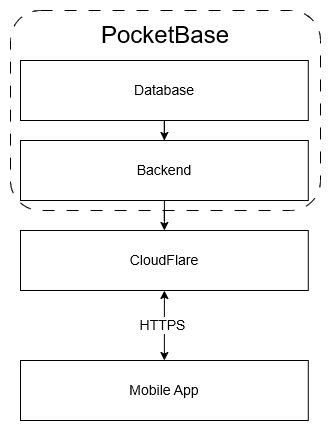
\includegraphics[width=0.5\textwidth]{assets/hla.png}
    \caption{Arsitektur Sistem}
\end{figure}

Client merepresentasikan seluruh aplikasi yang digunakan oleh \textit{end-user} atau pengguna, seperti aplikasi berbasis \textit{Mobile}, \textit{Website}, dsb\
untuk dapat menggunakan layanan yang disediakan oleh \textit{server}.

Server merepresentasikan seluruh komponen aplikasi yang dijalankan pada sisi \textit{server}.\
Hal ini meliputi \textit{Database}, dan \textit{Backend}. Pada sistem ini, seluruh fungsionalitas yang berkaitan dengan \textit{backend} dikelola \
sepenuhnya melalui \textit{framework} bernama PocketBase. PocketBase ini berjalan dalam server, dan dijalankan menggunakan aplikasi berbasis Go.\
Server juga dilindungi oleh Cloudflare, untuk perlindungan eksternal terhadap DDOS, yang juga berfungsi sebagai CDN untuk memperingan kinerja server dalam melayani \textit{request} dari \textit{client}.

\subsection{Arsitektur \textit{Database}}
Pada iterasi awal ini, Tembang Bali menyimpan seluruh data dalam 3 buah tabel, yaitu \textbf{songs}, \textbf{song\_types}, dan \textbf{song\_subtypes}.

\begin{figure}[H]
    \centering
    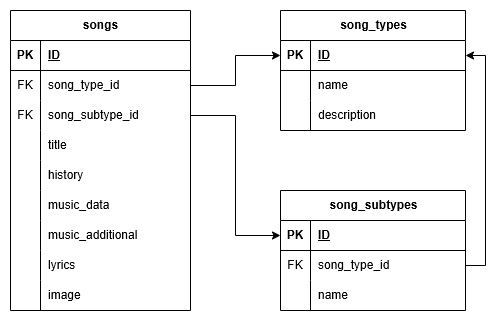
\includegraphics[width=0.8\textwidth]{assets/erd.png}
    \caption{ERD Database}
\end{figure}

\textbf{Tabel songs} terdiri atas \textit{column} \textit{song\_type\_id} dan \textit{song\_subtype\_id} yang berfungsi untuk menyimpan tipe dari data yang disimpan.\
\textit{Column} lainnya berfungsi sebagai \textit{metadata} dan juga lirik.
\textbf{Tabel song\_types} terdiri atas \textit{column} \textit{name} yang berisikan nama tipe dan \textit{description} yang berisi deskripsi singakt mengenai tipe dari data.\
\textbf{Tabel song\_sub\_types} terdiri atas \textit{column} \textit{name} yang berisikan nama tipe dan \textit{song\_type\_id} yang digunakan untuk menandakan relasi dengan \textbf{tabel song\_types}.\

\subsection{Arsitektur \textit{Mobile Client}}

\subsection{Arsitektur \textit{Keamanan}}
Pada iterasi ini, server Tembang Bali dapat diakses melalui domain yang dikelola menggunakan Cloudflare. Cloudflare digunakan untuk mencegah terjadinya serangan DDOS atau serangan lainnya yang memungkinkan terjadi pada server.
Pada iterasi selanjutnya, ketika sistem telah mengintegrasikan fitur-fitur yang memerlukan data pribadi milik user, data tersebut akan disimpan dalam bentuk yang telah terenkripsi, sehingga data tersebut hanya dapat diakses oleh pihak yang berwewenang.
API yang berhubungan dengan data pribadi juga akan memiliki fitur keamanan tersendiri, dan tidak dapat diakses dengan bebas tanpa adanya hak akses tertentu.
